%!TeX root=../sensetop.tex
\chapter[Chapter \thechapter]{}
\lettrine[lraise=0.3]{T}{he} first part of their journey was performed in too melancholy a disposition to be otherwise than tedious and unpleasant. But as they drew towards the end of it, their interest in the appearance of a country which they were to inhabit overcame their dejection, and a view of Barton Valley as they entered it gave them cheerfulness. It was a pleasant fertile spot, well wooded, and rich in pasture. After winding along it for more than a mile, they reached their own house. A small green court was the whole of its demesne in front; and a neat wicket gate admitted them into it.

As a house, Barton Cottage, though small, was comfortable and compact; but as a cottage it was defective, for the building was regular, the roof was tiled, the window shutters were not painted green, nor were the walls covered with honeysuckles. A narrow passage led directly through the house into the garden behind. On each side of the entrance was a sitting room, about sixteen feet square; and beyond them were the offices and the stairs. Four bed-rooms and two garrets formed the rest of the house. It had not been built many years and was in good repair. In comparison of Norland, it was poor and small indeed!—but the tears which recollection called forth as they entered the house were soon dried away. They were cheered by the joy of the servants on their arrival, and each for the sake of the others resolved to appear happy. It was very early in September; the season was fine, and from first seeing the place under the advantage of good weather, they received an impression in its favour which was of material service in recommending it to their lasting approbation.

The situation of the house was good. High hills rose immediately behind, and at no great distance on each side; some of which were open downs, the others cultivated and woody. The village of Barton was chiefly on one of these hills, and formed a pleasant view from the cottage windows. The prospect in front was more extensive; it commanded the whole of the valley, and reached into the country beyond. The hills which surrounded the cottage terminated the valley in that direction; under another name, and in another course, it branched out again between two of the steepest of them.

With the size and furniture of the house Mrs Dashwood was upon the whole well satisfied; for though her former style of life rendered many additions to the latter indispensable, yet to add and improve was a delight to her; and she had at this time ready money enough to supply all that was wanted of greater elegance to the apartments. <As for the house itself, to be sure,> said she, <it is too small for our family, but we will make ourselves tolerably comfortable for the present, as it is too late in the year for improvements. Perhaps in the spring, if I have plenty of money, as I dare say I shall, we may think about building. These parlours are both too small for such parties of our friends as I hope to see often collected here; and I have some thoughts of throwing the passage into one of them with perhaps a part of the other, and so leave the remainder of that other for an entrance; this, with a new drawing room which may be easily added, and a bed-chamber and garret above, will make it a very snug little cottage. I could wish the stairs were handsome. But one must not expect every thing; though I suppose it would be no difficult matter to widen them. I shall see how much I am before-hand with the world in the spring, and we will plan our improvements accordingly.>

In the mean time, till all these alterations could be made from the savings of an income of five hundred a-year by a woman who never saved in her life, they were wise enough to be contented with the house as it was; and each of them was busy in arranging their particular concerns, and endeavouring, by placing around them books and other possessions, to form themselves a home. Marianne's pianoforte was unpacked and properly disposed of; and Elinor's drawings were affixed to the walls of their sitting room.

In such employments as these they were interrupted soon after breakfast the next day by the entrance of their landlord, who called to welcome them to Barton, and to offer them every accommodation from his own house and garden in which theirs might at present be deficient. Sir John Middleton was a good looking man about forty. He had formerly visited at Stanhill, but it was too long for his young cousins to remember him. His countenance was thoroughly good-humoured; and his manners were as friendly as the style of his letter. Their arrival seemed to afford him real satisfaction, and their comfort to be an object of real solicitude to him. He said much of his earnest desire of their living in the most sociable terms with his family, and pressed them so cordially to dine at Barton Park every day till they were better settled at home, that, though his entreaties were carried to a point of perseverance beyond civility, they could not give offence. His kindness was not confined to words; for within an hour after he left them, a large basket full of garden stuff and fruit arrived from the park, which was followed before the end of the day by a present of game. He insisted, moreover, on conveying all their letters to and from the post for them, and would not be denied the satisfaction of sending them his newspaper every day.

% \begin{figure}[tbh]
% \centering
% 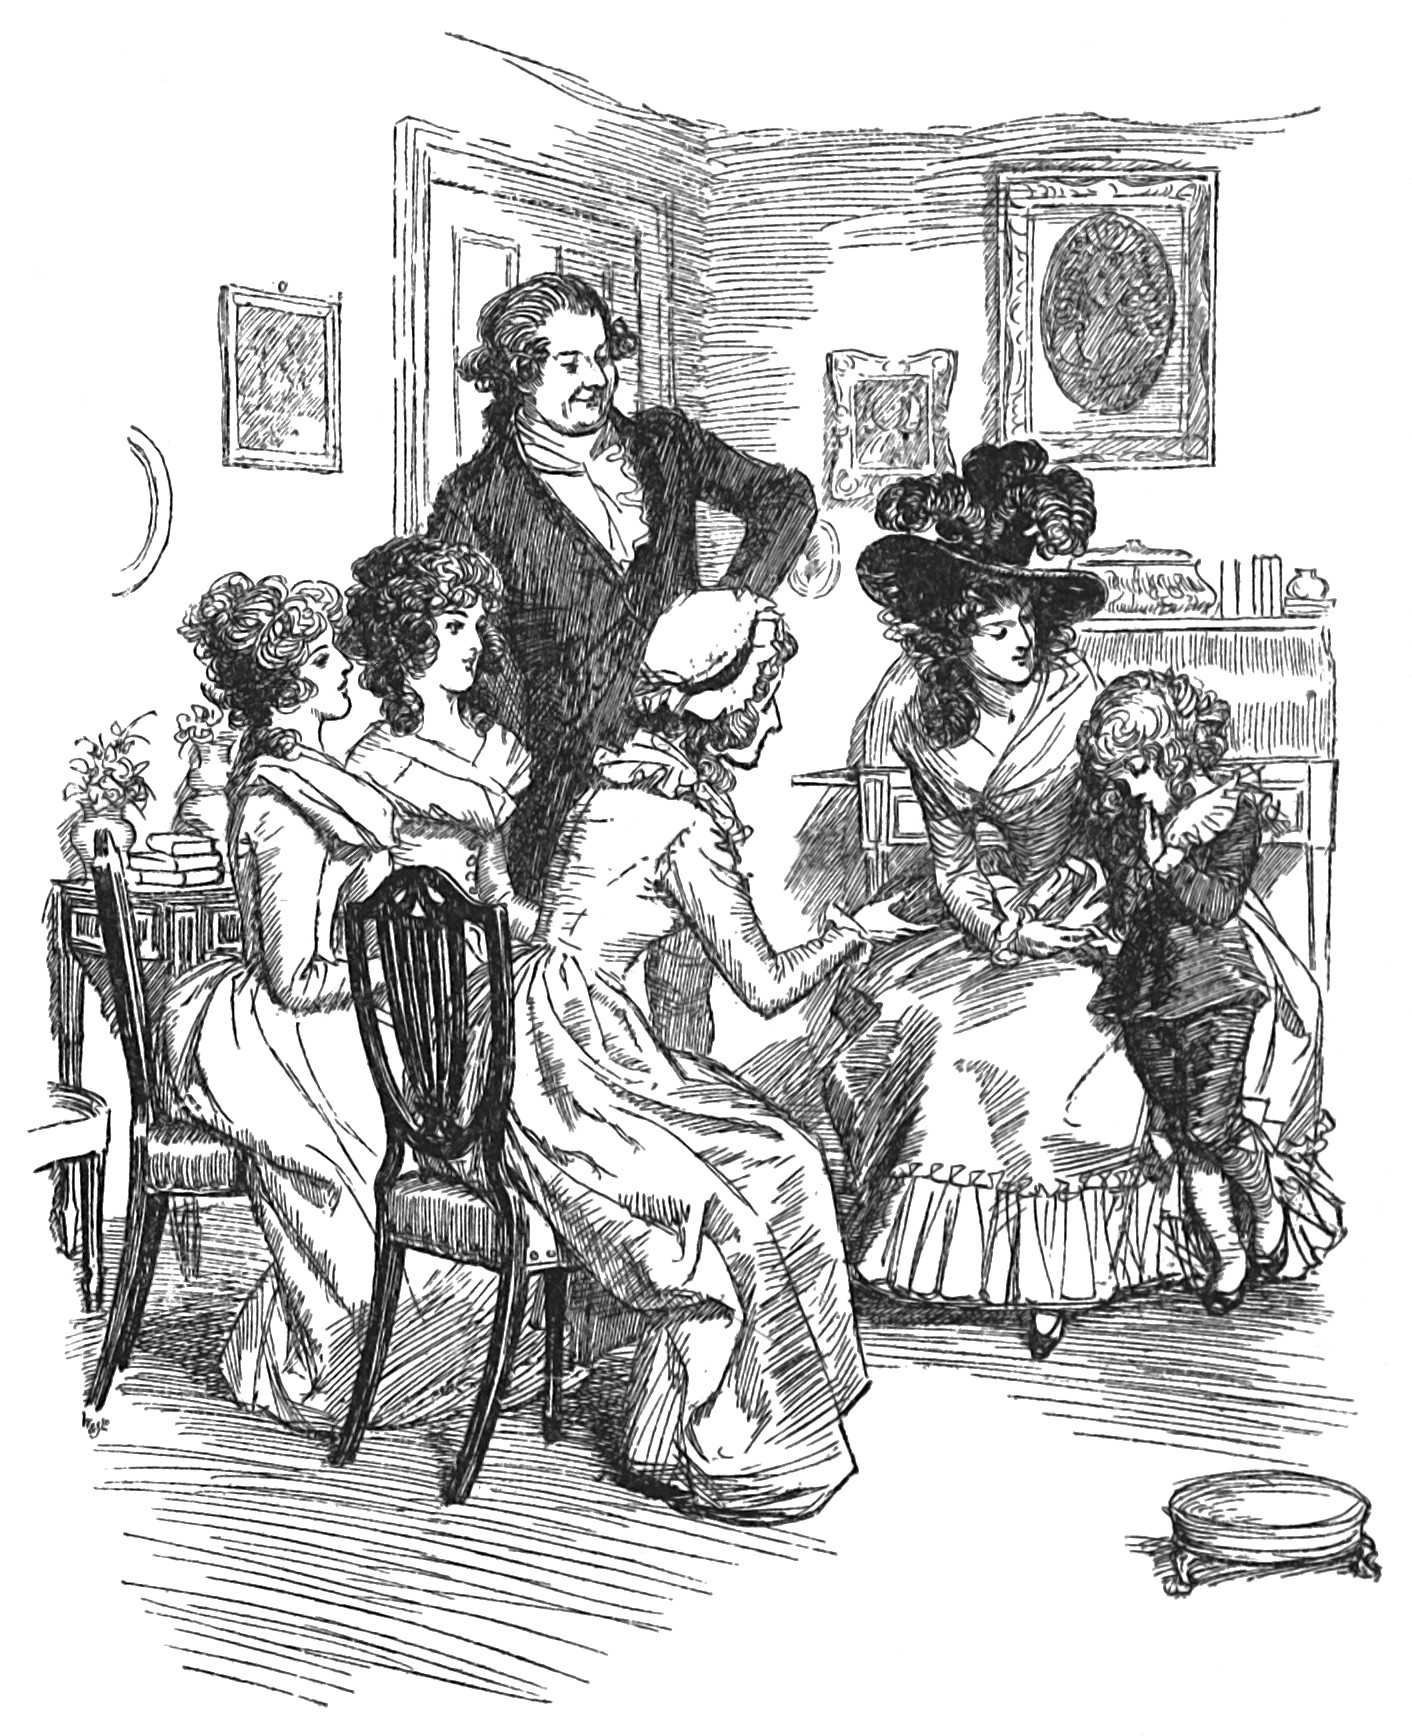
\includegraphics[width=\linewidth]{6shy}
% \caption{So shy before company}
% \end{figure}

\begin{bwbigpic}
	[1.0]
	{6shy} 
	{So shy before company} 
\end{bwbigpic}

Lady Middleton had sent a very civil message by him, denoting her intention of waiting on Mrs Dashwood as soon as she could be assured that her visit would be no inconvenience; and as this message was answered by an invitation equally polite, her ladyship was introduced to them the next day.

They were, of course, very anxious to see a person on whom so much of their comfort at Barton must depend; and the elegance of her appearance was favourable to their wishes. Lady Middleton was not more than six or seven and twenty; her face was handsome, her figure tall and striking, and her address graceful. Her manners had all the elegance which her husband's wanted. But they would have been improved by some share of his frankness and warmth; and her visit was long enough to detract something from their first admiration, by showing that, though perfectly well-bred, she was reserved, cold, and had nothing to say for herself beyond the most common-place inquiry or remark.

Conversation however was not wanted, for Sir John was very chatty, and Lady Middleton had taken the wise precaution of bringing with her their eldest child, a fine little boy about six years old, by which means there was one subject always to be recurred to by the ladies in case of extremity, for they had to enquire his name and age, admire his beauty, and ask him questions which his mother answered for him, while he hung about her and held down his head, to the great surprise of her ladyship, who wondered at his being so shy before company, as he could make noise enough at home. On every formal visit a child ought to be of the party, by way of provision for discourse. In the present case it took up ten minutes to determine whether the boy were most like his father or mother, and in what particular he resembled either, for of course every body differed, and every body was astonished at the opinion of the others.

An opportunity was soon to be given to the Dashwoods of debating on the rest of the children, as Sir John would not leave the house without securing their promise of dining at the park the next day.